\def\baselinestretch{1}
\chapter{Computing Reference Points $(Q_{H})$}
\section{Introduction to Reference Points}
\begin{definition}
 {\bf Reference Points:} are the discrete set of points on the edges of $\partial K_{i} \cap \partial G_{i}$  which are used to determine the
  half localization path of robot [see \cite{key5}].   
\end{definition}

\begin{definition}
 {\bf Half Localization Path:} is the path travelling along which the robot can eliminate half of the hypotheses by making
 observations at the reference points.
\end{definition}

For example,

\begin{figure}[h]
\begin{center}
\scalebox{0.50}{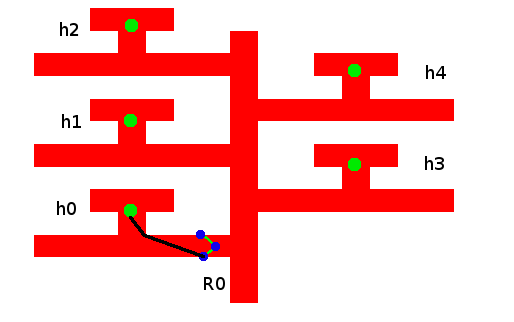
\includegraphics{Images/reference.png}}
\caption{\label{fig:Reference Points}Reference Points in blue color and hypotheses in green color}
\end{center}
\end{figure}

The reference points shown in the figure are for the hypothesis $h_0$. The robot on following the path from $h_0$ to $R_0$ 
can differentiate between hypotheses $\{h_0,h_1,h_2\}$ and $\{h_3, h_4\}$ based on its observation at $R_0$. The path shown in black is the half computing path.

\section{Algorithm}

\begin{enumerate}
 \item For every $i$ find those edges in $K_i$ which are not part of the boundary of majority map. These are important edges on which
we will find out reference points. Let $L_i$ contains all these edges for a particular $i$.
 \item  Calculate $r_0$(geodesic) radius of the smallest geodesic disk centered on $\gamma_{0}$ that intersects at least half of $L_{i}'s$.
\begin{enumerate}
 \item For all $i$ calculate the minimum distance between $\gamma_{0}$ and any of the line segments of $L_i$.
 \item Take the median of all the distances calculated above as the geodesic radius$(r_0)$. 
\end{enumerate}
 \item Let $k$ be the number of hypotheses and $R$ be a sequence of radii $r_0,2*r_0,4*r_0 \dots , 2^{\lceil \log_{2}k \rceil}$.
 \item For every hypothesis $i$ perform the following steps
\begin{enumerate}
 \item Place each line segment $\sigma$ in $L_i$ on an axis aligned square centered at $\gamma_{0}$ of side length $2*2^{j}*r_0$ (where $j$ from $(0..\lceil \log_{2}k \rceil)$)
 \item Decompose the square into $kxk$ grid using $k-1$ horizontal and vertical lines.
 \item Calculate the intersection of the line segment with the grid line. These intersection points are the reference points. Also include 
 end points of the line segment(even if they do not lie on grid) in the set of reference points.  
\end{enumerate}

\end{enumerate}

\section{Examples}

\begin{figure}
\begin{center}
\scalebox{0.60}{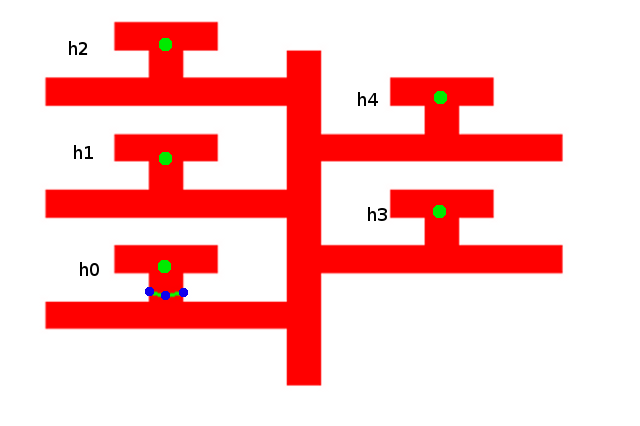
\includegraphics{Images/reference1.png}}
\caption{\label{fig:Construction}Reference Points in blue color and hypotheses in green color}
\end{center}
\end{figure}

\begin{figure}
\begin{center}
\scalebox{0.40}{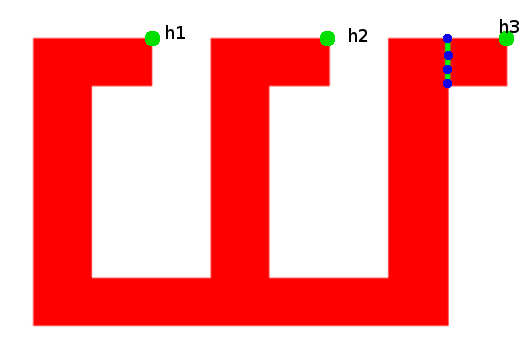
\includegraphics{Images/reference2.png}}
\caption{\label{fig:Construction}Reference Points in blue color and hypotheses in green color}
\end{center}
\end{figure}





%%% ----------------------------------------------------------------------

% ------------------------------------------------------------------------

%%% Local Variables: 
%%% mode: latex
%%% TeX-master: "../thesis"
%%% End: 
